%%%%%%%%%%%%%%%%%%%%%%%%%%%%%%%%%%%%%%%%%
% FRI Data Science_report LaTeX Template
% Version 1.0 (28/1/2020)
%
% Jure Demšar (jure.demsar@fri.uni-lj.si)
%
% Based on MicromouseSymp article template by:
% Mathias Legrand (legrand.mathias@gmail.com)
% With extensive modifications by:
% Antonio Valente (antonio.luis.valente@gmail.com)
%
% License:
% CC BY-NC-SA 3.0 (http://creativecommons.org/licenses/by-nc-sa/3.0/)
%
%%%%%%%%%%%%%%%%%%%%%%%%%%%%%%%%%%%%%%%%%


%----------------------------------------------------------------------------------------
%	PACKAGES AND OTHER DOCUMENT CONFIGURATIONS
%----------------------------------------------------------------------------------------
\documentclass[fleqn,moreauthors,10pt]{ds_report}
\usepackage[english]{babel}
\usepackage{numprint}

\graphicspath{{fig/}}




%----------------------------------------------------------------------------------------
%	ARTICLE INFORMATION
%----------------------------------------------------------------------------------------

% Header
\JournalInfo{UL FRI Data Science - Natural Language Processing, 2021-2022}

% Interim or final report
\Archive{Interim report}
%\Archive{Project Report}

% Article title
\PaperTitle{Literacy situation models knowledge base creation}

% Authors and their info
%\Authors{John Doe\textsuperscript{1}}
%\affiliation{\textsuperscript{1}\textit{john.doe@fri.uni-lj.si, 63181234}}

% Multiple authors
\Authors{Uroš Škrjanc\textsuperscript{1}, Matthew Tanti\textsuperscript{2}, and Marko Novak\textsuperscript{3}}
\affiliation{\textsuperscript{1}\textit{us1883@student.uni-lj.si, 63030323}}
\affiliation{\textsuperscript{2}\textit{mt9734@student.uni-lj.si, 63210511}}
\affiliation{\textsuperscript{3}\textit{mn3983@student.uni-lj.si, 63130166}}

% Keywords
\Keywords{story entities, family relationship extraction, short stories}
\newcommand{\keywordname}{Keywords}


%----------------------------------------------------------------------------------------
%	ABSTRACT
%----------------------------------------------------------------------------------------

\Abstract{
%The abstract goes here. The abstract goes here. The abstract goes here. The abstract goes here. The abstract goes here. The abstract goes here. The abstract goes here. The abstract goes here. The abstract goes here. The abstract goes here. The abstract goes here. The abstract goes here. The abstract goes here. The abstract goes here. The abstract goes here. The abstract goes here. The abstract goes here. The abstract goes here. The abstract goes here. The abstract goes here. The abstract goes here. The abstract goes here. The abstract goes here. The abstract goes here. The abstract goes here. The abstract goes here.
}

%----------------------------------------------------------------------------------------

\begin{document}

% Makes all text pages the same height
\flushbottom

% Print the title and abstract box
\maketitle

% Removes page numbering from the first page
\thispagestyle{empty}

%----------------------------------------------------------------------------------------
%	ARTICLE CONTENTS
%----------------------------------------------------------------------------------------

\section*{Introduction}

The field of recognising the content and structure of texts and extracting content from them is increasingly related to machine learning methods. Not only syntax checking but also pure understanding of texts by humans is interesting for machine learning for different motives. There is practically no more field related to language that in some way could not be linked to machine learning methods.



%These latex files are intended to serve as a the template for the FRI Data Science Project Competition. If you find mistakes in the template or have problems using it, please consult Jure Demšar (\href{mailto:jure.demsar@fri.uni-lj.si}{jure.demsar@fri.uni-lj.si}).

%In the Introduction section you should write about the relevance of your work (what is the purpose of the project, what will we solve) and about related work (what solutions for the problem already exist). Where appropriate, reference scientific work conducted by other researchers. For example, the work done by Demšar et al. \cite{Demsar2016BalancedMixture} is very important for our project. The abbreviation et al. is for et alia, which in latin means and others, we use this abbreviation when there are more than two authors of the work we are citing. If there are two authors (or if there is a single author) we just write down their surnames. For example, the work done by Demšar and Lebar Bajec \cite{Demsar2017LinguisticEvolution} is also important for successful completion of our project.


%------------------------------------------------

\subsection*{Related Work}

J. Leng and P. Jiang explored relationship extraction using a deep learning approach to help support decision making in a social manufacturing context. This paper focused on creating a deep learning model that is based on an improved stacked denoising auto-encoder on sentence-level features. This model extracts manufacturing relationships, named entities, and text-based contexts. Their results reveal that this approach produces similar performance to the latest learning models.~\cite{leng2016deep}

C. Giles and J. Wren developed an SVM classifier using NLP-based approaches to extract relationships between entities such as genes, chemicals, metabolites, phenotypes, and diseases. The classifier would label what kind of relationship there is between two entities, such as positive or negative, then detect what type of semantic relationship they have, such as binds, cleaves, etc. The main goal of this paper was to get the highest accuracy possible to prevent contradictions, but some inaccuracy was expected. SVM cross-validation showed that the implementation had a good F1 score at \numprint{88}\%.~\cite{giles2008large}

A. Roberts et al. worked on a supervised machine learning system (SVM) which was trained on a corpus of patient narratives which were manually annotated with clinical relationships. To evaluate the model, a standard ten-fold cross-validation methodology and standard evaluation metrics were used. This resulted in an F1 score of \numprint{75}\%. The paper concluded that it is possible to extract (clinical) relationships from text using an SVM with shallow features. ~\cite{roberts2008extracting}

V. Devisree and PC. Reghu Raj combined the unsupervised and supervised approaches to create a hybrid model that is able to extract relationships from stories. The model identifies the main characters, collects sentences that relate to them, then these sentences are analysed, and finally, the relationship between the characters is classified. Whilst training, if the sentence is classified, then it goes through the supervised section of the model, and if it's unclassified, it goes through the unsupervised section of the model.l The corpus used was a set of \numprint{100} short stories for kids, which contained multiple different relationship types. Three relationship categories were used; Parent-Child, Friendship, and No-Relation, the hybrid model managed to achieve an F1 score of \numprint{83}\%  ~\cite{devisree2016hybrid}.

\section*{Methods}

In the group, we decided to try to analyse different short stories to extract information about the characters who appear in the texts and to find out what kind of relationships these characters are in.

First, we found a collection of English short stories and chose a subset of them for training. We took two datasets of stories, both based on data from Project Gutenberg. We used NLTK to split each story into sentences and selected the stories with at most \numprint{1000} sentences. Then we used spaCy's English language model to tokenise the sentences and search each story for words indicating family relationships. We calculated the average number of such words per sentence and selected only the stories where at least \numprint{5}\% of sentences contain such words.

This resulted in a total of \numprint{96} candidate stories; however, not all of them were suitable as they didn't contain many named characters. Such stories might, for example, contain references to the mother or father of the main character but never state their names. That's why we took spaCy's transformer-based English language model to do NER (named entity recognition) and filter out the stories with less than \numprint{4} named persons.

In the end, we got \numprint{47} short stories and a rough list of recognised persons for each story. The goal was first to improve the NER model to fix incorrect labels and detect the "poetic names," e.g. when a person is referred to as "the Bearded One" throughout the story. Then we needed to group all names belonging to the same person, and add the data about family relationships, so it would be suitable for training DocRed~\cite{yao2019DocRED}-derived models for document-level relation extraction, such as DocuNet~\cite{ijcai2021-551}.

%Use the Methods section to describe what you did an how you did it -- in what way did you prepare the data, what algorithms did you use, how did you test various solutions ... Provide all the required details for a reproduction of your work.

%Below are \LaTeX examples of some common elements that you will probably need when writing your report (e.g. figures, equations, lists, code examples ...).

%\section*{Existing solutions}

%The use of deep neural networks is on the rise in already implemented solutions, but other approaches and combinations of these are also used in models for classifying family relations between persons in the text, such as rule-based approaches, utterance attribution and vocative detection technique and unsupervised approach to the extraction of interpersonal relations are described in the articles, which we intend to take as a basis for further work.

%\section*{Relations}

%We decided to check if the following relations occur between the character in short stories:

% \begin{itemize}
% \itemsep0em
% \item Wife
% \item Husband
% \item Mother
% \item Father
% \item Daughter
% \item Son
% \item Sister
% \item Brother
% \item Grandmother
% \item Grandfather
% \item Granddaughter
% \item Grandson
% \item Mother-in-law
% \item Father-in-law
% \item Daughter-in-law
% \item Son-in-law
% \item Sister-in-law
% \item Brother-in-law
% \item Aunt
% \item Uncle
% \item Niece
% \item Nephew
% \item Cousin
% \end{itemize}

% Those are the broadest family relations we intend to use. We expect that there will be no need to add new relationships. If the model proves to be too large for our task, some relations can be removed from the model.

\subsection*{Data preparation}

We used Prodigy to improve data annotation, as it's aimed to complement spaCy, and it offers a really simple UI as well as on-line model training for semi-supervised data annotation. The resulting model can then directly be used with spaCy on new data.

Stories generally don't explicitly state relationships between persons in a single sentence; it's much more common for the relationships to be evident from several indirect sentences. That's why it's necessary to label such indirect sentences as "evidence" of a relationship between two persons. That's why the final dataset we prepared contains tokenised sentences, named entities (persons) and all different names each entity is referred to in the text, relationships between those entities, and finally, which sentences serve as evidence of such relationships.

\section*{Results}

The resulting NER model achieved accuracy above \numprint{90}\% on the stories, which is a significant improvement over \numprint{67}\% achieved by spaCy's RoBERTa-based model for the English language.

The final relation extraction model, however, wasn't able to achieve the expected results, as it quickly started overfitting due to a relatively small dataset and only achieved the best F1 score of \numprint{4}\%.

%------------------------------------------------

\section*{Discussion}

Clearly, a dataset of \numprint{47} stories isn't sufficient to train a large NLP model, and significantly more data would be needed to achieve a sufficient improvement or come close to the state-of-the-art models for document-level relation extraction of over \numprint{60}\%. To speed up data annotation for such a dataset, it would make sense to define a custom config for Prodigy where all labelling could be done in a single step; however, for our purposes and the scale of the problem, it would take longer to do that than it did to do the last step of labelling manually in a text editor.

%\subsection*{Equations}

% You can write equations inline, e.g. $\cos\pi=-1$, $E = m \cdot c^2$ and $\alpha$, or you can include them as separate objects. The Bayes’s rule is stated mathematically as:

% \begin{equation}
%     P(A|B) = \frac{P(B|A)P(A)}{P(B)},
%     \label{eq:bayes}
% \end{equation}

% where $A$ and $B$ are some events. You can also reference it -- the equation \ref{eq:bayes} describes the Bayes's rule.

% \subsection*{Lists}

% We can insert numbered and bullet lists:

% the [noitemsep] option makes the list more compact
% \begin{enumerate}[noitemsep]
%     \item First item in the list.
%     \item Second item in the list.
%     \item Third item in the list.
% \end{enumerate}

% \begin{itemize}[noitemsep]
%     \item First item in the list.
%     \item Second item in the list.
%     \item Third item in the list.
% \end{itemize}

% We can use the description environment to define or describe key terms and phrases.

% \begin{description}
%     \item[Word] What is a word?.
%     \item[Concept] What is a concept?
%     \item[Idea] What is an idea?
% \end{description}


% \subsection*{Random text}

% This text is inserted only to make this template look more like a proper report. Lorem ipsum dolor sit amet, consectetur adipiscing elit. Etiam blandit dictum facilisis. Lorem ipsum dolor sit amet, consectetur adipiscing elit. Interdum et malesuada fames ac ante ipsum primis in faucibus. Etiam convallis tellus velit, quis ornare ipsum aliquam id. Maecenas tempus mauris sit amet libero elementum eleifend. Nulla nunc orci, consectetur non consequat ac, consequat non nisl. Aenean vitae dui nec ex fringilla malesuada. Proin elit libero, faucibus eget neque quis, condimentum laoreet urna. Etiam at nunc quis felis pulvinar dignissim. Phasellus turpis turpis, vestibulum eget imperdiet in, molestie eget neque. Curabitur quis ante sed nunc varius dictum non quis nisl. Donec nec lobortis velit. Ut cursus, libero efficitur dictum imperdiet, odio mi fermentum dui, id vulputate metus velit sit amet risus. Nulla vel volutpat elit. Mauris ex erat, pulvinar ac accumsan sit amet, ultrices sit amet turpis.

% Phasellus in ligula nunc. Vivamus sem lorem, malesuada sed pretium quis, varius convallis lectus. Quisque in risus nec lectus lobortis gravida non a sem. Quisque et vestibulum sem, vel mollis dolor. Nullam ante ex, scelerisque ac efficitur vel, rhoncus quis lectus. Pellentesque scelerisque efficitur purus in faucibus. Maecenas vestibulum vulputate nisl sed vestibulum. Nullam varius turpis in hendrerit posuere.


% \subsection*{Figures}

% You can insert figures that span over the whole page, or over just a single column. The first one, \figurename~\ref{fig:column}, is an example of a figure that spans only across one of the two columns in the report.

% \begin{figure}[ht]\centering
%     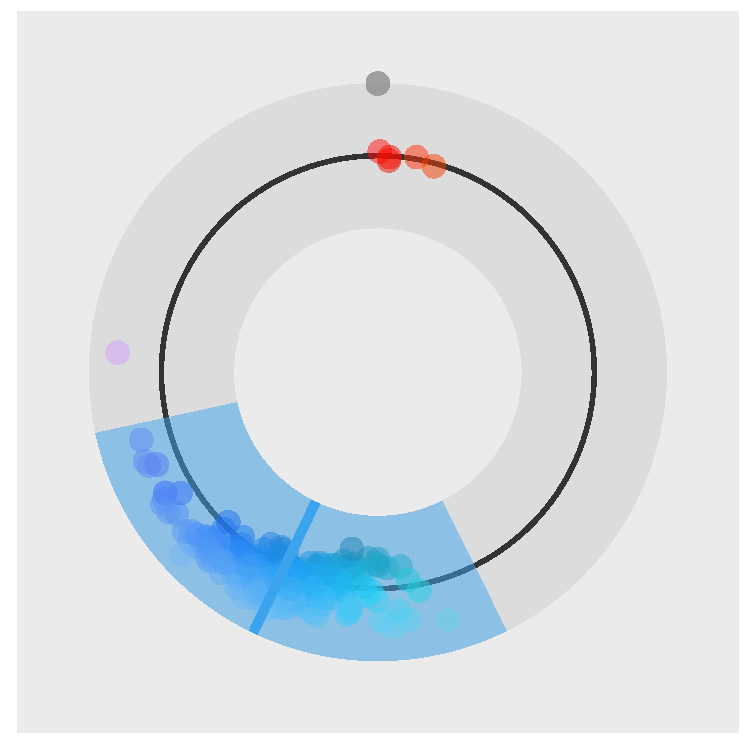
\includegraphics[width=\linewidth]{single_column.pdf}
%     \caption{\textbf{A random visualization.} This is an example of a figure that spans only across one of the two columns.}
%     \label{fig:column}
% \end{figure}

% On the other hand, \figurename~\ref{fig:whole} is an example of a figure that spans across the whole page (across both columns) of the report.

% \begin{figure*} makes the figure take up the entire width of the page
% \begin{figure*}[ht]\centering
%     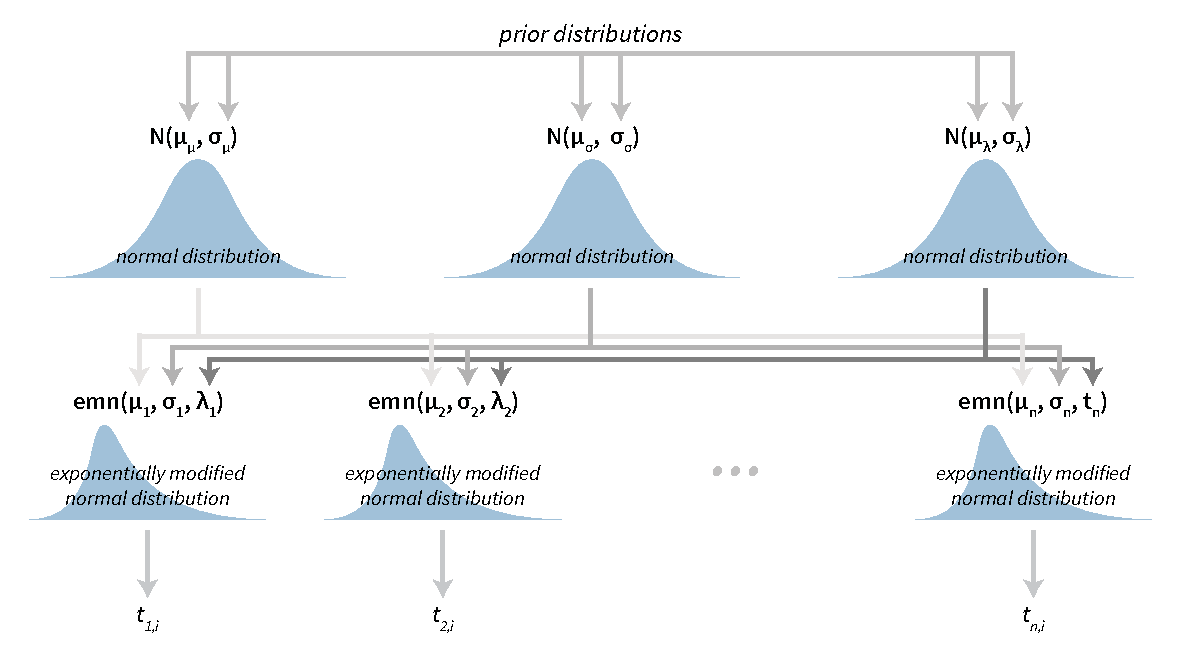
\includegraphics[width=\linewidth]{whole_page.pdf}
%     \caption{\textbf{Visualization of a Bayesian hierarchical model.} This is an example of a figure that spans the whole width of the report.}
%     \label{fig:whole}
% \end{figure*}


% \subsection*{Tables}

% Use the table environment to insert tables.

% \begin{table}[hbt]
%     \caption{Table of grades.}
%     \centering
%     \begin{tabular}{l l | r}
%         \toprule
%         \multicolumn{2}{c}{Name}       \\
%         \cmidrule(r){1-2}
%         First name & Last Name & Grade \\
%         \midrule
%         John       & Doe       & $7.5$ \\
%         Jane       & Doe       & $10$  \\
%         Mike       & Smith     & $8$   \\
%         \bottomrule
%     \end{tabular}
%     \label{tab:label}
% \end{table}


% \subsection*{Code examples}

% You can also insert short code examples. You can specify them manually, or insert a whole file with code. Please avoid inserting long code snippets, advisors will have access to your repositories and can take a look at your code there. If necessary, you can use this technique to insert code (or pseudo code) of short algorithms that are crucial for the understanding of the manuscript.

% \lstset{language=Python}
% \lstset{caption={Insert code directly from a file.}}
% \lstset{label={lst:code_file}}
% \lstinputlisting[language=Python]{code/example.py}

% \lstset{language=R}
% \lstset{caption={Write the code you want to insert.}}
% \lstset{label={lst:code_direct}}
% \begin{lstlisting}
% import(dplyr)
% import(ggplot)

% ggplot(diamonds,
% 	   aes(x=carat, y=price, color=cut)) +
%   geom_point() +
%   geom_smooth()
% \end{lstlisting}

%------------------------------------------------

% \section*{Results}

% Use the results section to present the final results of your work. Present the results in a objective and scientific fashion. Use visualisations to convey your results in a clear and efficient manner. When comparing results between various techniques use appropriate statistical methodology.

% \subsection*{More random text}

% This text is inserted only to make this template look more like a proper report. Lorem ipsum dolor sit amet, consectetur adipiscing elit. Etiam blandit dictum facilisis. Lorem ipsum dolor sit amet, consectetur adipiscing elit. Interdum et malesuada fames ac ante ipsum primis in faucibus. Etiam convallis tellus velit, quis ornare ipsum aliquam id. Maecenas tempus mauris sit amet libero elementum eleifend. Nulla nunc orci, consectetur non consequat ac, consequat non nisl. Aenean vitae dui nec ex fringilla malesuada. Proin elit libero, faucibus eget neque quis, condimentum laoreet urna. Etiam at nunc quis felis pulvinar dignissim. Phasellus turpis turpis, vestibulum eget imperdiet in, molestie eget neque. Curabitur quis ante sed nunc varius dictum non quis nisl. Donec nec lobortis velit. Ut cursus, libero efficitur dictum imperdiet, odio mi fermentum dui, id vulputate metus velit sit amet risus. Nulla vel volutpat elit. Mauris ex erat, pulvinar ac accumsan sit amet, ultrices sit amet turpis.

% Phasellus in ligula nunc. Vivamus sem lorem, malesuada sed pretium quis, varius convallis lectus. Quisque in risus nec lectus lobortis gravida non a sem. Quisque et vestibulum sem, vel mollis dolor. Nullam ante ex, scelerisque ac efficitur vel, rhoncus quis lectus. Pellentesque scelerisque efficitur purus in faucibus. Maecenas vestibulum vulputate nisl sed vestibulum. Nullam varius turpis in hendrerit posuere.

% Nulla rhoncus tortor eget ipsum commodo lacinia sit amet eu urna. Cras maximus leo mauris, ac congue eros sollicitudin ac. Integer vel erat varius, scelerisque orci eu, tristique purus. Proin id leo quis ante pharetra suscipit et non magna. Morbi in volutpat erat. Vivamus sit amet libero eu lacus pulvinar pharetra sed at felis. Vivamus non nibh a orci viverra rhoncus sit amet ullamcorper sem. Ut nec tempor dui. Aliquam convallis vitae nisi ac volutpat. Nam accumsan, erat eget faucibus commodo, ligula dui cursus nisi, at laoreet odio augue id eros. Curabitur quis tellus eget nunc ornare auctor.

% Phasellus in ligula nunc. Vivamus sem lorem, malesuada sed pretium quis, varius convallis lectus. Quisque in risus nec lectus lobortis gravida non a sem. Quisque et vestibulum sem, vel mollis dolor. Nullam ante ex, scelerisque ac efficitur vel, rhoncus quis lectus. Pellentesque scelerisque efficitur purus in faucibus. Maecenas vestibulum vulputate nisl sed vestibulum.


%------------------------------------------------

% \section*{Acknowledgments}

% Here you can thank other persons (non-authors) that contributed to the successful completion of your project.


%----------------------------------------------------------------------------------------
%	REFERENCE LIST
%----------------------------------------------------------------------------------------
\bibliographystyle{unsrt}
\bibliography{report}


\end{document}
